\documentclass{bredelebeamer}

% Customs:
\usepackage[utf8]{inputenc}
\usepackage{amsmath,amsfonts,amssymb,graphicx}
\usepackage[document]{ragged2e}
\usepackage[Euler]{upgreek}

% Define mathbfit
\DeclareMathAlphabet{\mathbfit}{OML}{cmm}{b}{it}
\DeclareMathAlphabet{\mathbfsf}{\encodingdefault}{\sfdefault}{bx}{n}

\usepackage[backend=biber]{biblatex}
\addbibresource{ref.bib}

% Setting graphics path
\graphicspath{{./rsc/}{./rsc/pdf/}{./rsc/svg/}{./rsc/image/}}

% Define operators
\DeclareMathOperator*{\argmax}{arg\,max}
\DeclareMathOperator*{\argmin}{arg\,min}
\DeclareMathOperator*{\minimize}{Minimize}
\DeclareMathOperator*{\maximize}{Maximize}

\DeclareMathOperator*{\E}{\mathbb{E}}
\DeclareMathOperator*{\var}{Var}

% Define textbfit
\makeatletter
\DeclareRobustCommand\bfseriesitshape{
  \not@math@alphabet\itshapebfseries\relax
  \fontseries\bfdefault
  \fontshape\itdefault
  \selectfont
}
\makeatother
\DeclareTextFontCommand{\textbfit}{\bfseriesitshape}

\usefonttheme[onlymath]{serif}

%%%%%%%%%%%%%%%%%%%%%%%%%%%%%%%%%%%%%%%%%%%%%%%% META DATA start

\title[ML Basics]{Sampling 2}
% Titre du diaporama

\subtitle{A self-study metarials for PRML~\cite{bishop:2006:PRML}}
% Sous-titre optionnel

\author{Jisung Lim\inst{1}}
% The \inst {...} command displays the member's affiliation.
% If there are several speakers: Marcel Dupont \inst {1}, Roger Durand
% \inst {2} Simply add another institute on the model below.

\institute[Yonsei]
{
  \inst{1}%
  B.S. Candidate of Industrial Engineering\\
  Yonsei University, South Korea.
}

\date{24th June, 2017}
% Optional. The date, usually the day of the conference.

\subject{Sampling and MCMC 2.}
% This is used in the pdf metadata

\logo{
  \begin{tikzpicture}
    \pgfmathsetmacro{\myopacity}{0.25}
    \node[opacity=\myopacity] {
      
\includegraphics[scale=0.08]{yonsei_emblem.png}
      
\includegraphics[scale=0.08]{yonsei_logo_text.png}
    };
  \end{tikzpicture}
}

%%%%%%%%%%%%%%%%%%%%%%%%%%%%%%%%%%%%%%%%%%%%%%%% META DATA end

%%%%%%%%%%%%%%%%%%%%%%%%%%%%%%%%%%%%%%%%%%%%%%%% DOCUMENT start

\begin{document}

%%%%%%%%%%%%%%%%%%%%%%%%%%%%%%%%%%%%%%%%%%%%%%%%%%%%%%%%%%% TITLE PAGE

\begin{frame}
  \titlepage
\end{frame}

\printbibliography
%%%%%%%%%%%%%%%%%%%%%%%%%%%%%%%%%%%%%%%%%%%%%%%%%%%%%%%%%%% SUMMARY

\begin{frame}{Summary}
  \tableofcontents
  % Option to add option [pausesections]
\end{frame}

%%%%%%%%%%%%%%%%%%%%%%%%%%%%%%%%%%%%%%%%%%%%%%%%%%%%%%%%%%%%%%%%%%%%%
\section{Introduction}
\subsection{Metropolis Algorithm}
\begin{frame}{Metropolis Algorithm}
  \textbf{State:}
  \begin{itemize}
    \item $\mathbfit{z}^{(1)}$, $\mathbfit{z}^{(2)}$, \ldots forms Markov chain
  \end{itemize}
  \begin{equation}
    \textrm{current state: } \mathbfit{z}^{(\tau)}
  \end{equation}

  \textbf{Proposal distribution at $\tau$:}
  \begin{itemize}
    \item It should be simple enough to draw sample directly.
    \item Symmetry condition:
    $q(\mathbfit{z}|\mathbfit{z}') = q(\mathbfit{z}'|\mathbfit{z})$
  \end{itemize}
  \begin{equation}
    \textrm{proposal distribution: } q(\mathbfit{z}|\mathbfit{z}^{(\tau)})
  \end{equation}

  \textbf{True distribution:}
  \begin{itemize}
    \item tractable up to its normalization term
  \end{itemize}
  \begin{equation}
    \textrm{true distribution: } p(\mathbfit{z}) = \tilde{p}(\mathbfit{z})/Z_p
  \end{equation}
\end{frame}

\begin{frame}{Metropolis Algorithm}
  \textbf{Algorithm:}
  At each cycle of the algorithm,
  \begin{enumerate}
    \item We generate a candidate sample $\mathbfit{z}^{(*)}$
    from the proposal distribution.
    \item and then accept the sample according to an appropriate criterion.
    \\[2.0\baselineskip]
  \end{enumerate}

  \textbf{Acceptance function:}
  \begin{equation}
    A(\mathbfit{z}^{*}, \mathbfit{z}^{(\tau)})
    = \min( 1, a(\tau) )
    \quad \text{where} \quad a(\tau) =
    \frac{\tilde{p}(\mathbfit{z}^{*})}
    {\tilde{p}(\mathbfit{z}^{(\tau)})}
  \end{equation}

  \textbf{Rejection criterion:}
  \begin{equation}
    \begin{split}
      \textrm{Reject: } &A(\mathbfit{z}^{*}, \mathbfit{z}^{(\tau)}) \leq u(0,1) \\
      \textrm{Accept: } &A(\mathbfit{z}^{*}, \mathbfit{z}^{(\tau)}) > u(0,1)
    \end{split}
  \end{equation}
  where $u$ is randomly picked from uniform distribution $U(0,1)$.
\end{frame}


\section{Markov Chain}
\subsection{Markov Chain}
\begin{frame}{Markov Chain; Definition}
  Before discussing MCMC methods, it is fair to study some general and useful
  properties of Markov chains in some detail. We only deals with first-order
  Markov chain in this chapter which is defined by
  \begin{definition}
    A first-order Markov Chain is defined to be a series of \textbf{random variables}
    \begin{equation}
      \mathbfit{z}^{(1)}, \ldots, \mathbfit{z}^{(M)}
    \end{equation}
    satisfying the Markov property given by
    \begin{equation*}
      p(\mathbfit{z}^{(m+1)}|\mathbfit{z}^{(1)}, \ldots, \mathbfit{z}^{(m)})
      = p(\mathbfit{z}^{(m+1)}|\mathbfit{z}^{(m)})
    \end{equation*}
  \end{definition}
  which also can be represented as a directed graph in the form of a chain.
  And the finite-dimensional (here, it stands for time dimension) is given by
  \begin{equation}
    P (\mathbfit{z}^{(1)}, \ldots, \mathbfit{z}^{(M)})
  \end{equation}

\end{frame}

\begin{frame}{Markov Chain; Examining the state space}
  \textit{General definition of Stochastic process}
  \begin{equation}
    X : (\Omega, \mathcal{F}) \rightarrow (S^{\infty},\mathcal{E}^{\infty})
  \end{equation}
  where $(S, \mathcal{E})$ is state space on which $X^{(n)}$'s are defined as
  follows
  \begin{equation}
    X^{(n)} :  (\Omega, \mathcal{F}) \rightarrow (S, \mathcal{E})
  \end{equation}

  \textit{The random variable from State space to Sampling space}
  The stochastic process, or discrete-time Markov chain, have countable
  state space $S$. To simplify the notation and focus on the sample itself
  we introduce the random vector maps original state $S$ to $\mathbf{z}$ which
  is equiprobable, $D$-dimensional space.
  \begin{equation}
    \mathbf{z}^{(n)}: (S, \mathcal{E}) \rightarrow (\mathbf{z}, \mathcal{A})
  \end{equation}
  where $\mathcal{A}$ is a $\sigma$-algebra of $\mathbf{z}$.
\end{frame}


\begin{frame}{Markov Chain; Properties}
  \begin{itemize}
    \item \textit{Initial state}: $\mathbfit{z}^{(0)}$
    \item \textit{Transition probability}:
    \begin{equation}
      T_m(\mathbfit{z}^{(m)},\mathbfit{z}^{(m+1)})
      := p(\mathbfit{z}^{(m+1)}|\mathbfit{z}^{(m)})
    \end{equation}
    \item \textit{Time homogenuity}:
    \begin{equation}
      T_m(\mathbfit{z}^{(m)},\mathbfit{z}^{(m+1)})
      = T_n(\mathbfit{z}^{(n)},\mathbfit{z}^{(n+1)})
      \quad \forall m, n
    \end{equation}
    \item \textit{Invariant distribution:}
    \begin{equation}
      p(\mathbfit{z}) = \sum_{\mathbfit{z}'} T(\mathbfit{z}',\mathbfit{z}) p(\mathbfit{z}')
    \end{equation}
    \item \textit{Detailed balance:}
    \begin{equation}
      p(\mathbfit{z}) T(\mathbfit{z},\mathbfit{z}')
      = p(\mathbfit{z}') T(\mathbfit{z}',\mathbfit{z})
    \end{equation}
  \end{itemize}
\end{frame}

\begin{frame}{Markov Chain; properties}
  \textbf{Properties}
  From the definition and the specification of the first-order Markov chain,
  we can examine some useful properties.
  \begin{itemize}
    \item \textit{Reducibility}:
    A Markov chain is said to be irreducible if it is possible to get
    to any state from any state. The accessibility can be defined by
    \begin{equation}
      P(\mathbfit{z}_{n} | \mathbfit{z}_{m}) > 0 \quad \forall n, m
    \end{equation}
    \item \textit{Periodicity}:
    A state $n$ has period $p$ if any return to state $n$ must occur in
    multiples of $p$ time steps. If $p = 1$, then the state is said to
    be \textit{aperiodic}.
    \item \textit{Recurrent}:
    A state $n$ is said to be \textit{transient} if, given that we start
    in state $n$, there is a non-zero probability that we will never
    return to $n$. State $n$ is \textit{recurrent} (or persistent) if
    it is not transient.
    \item \textit{Ergodicity}:
    The Markov chain is called ergodic if it is irreducible, and its
    states are positive recurrent and aperiodic.
  \end{itemize}
\end{frame}

\subsection{Markov Chain for MCMC}
\begin{frame}{Markov Chain for MCMC}
  \textbf{Our goal} is still to generate a sample from $p(\mathbfit{z})$.
  \begin{itemize}
    \item A standard Markov chain Monte Carlo approach is to construct
    an \textbfit{ergodic} Markov chain with a stationary distribution.
  \end{itemize}

  The main properties underpinning the MCMC method, to accomplish our goal,
  are followings.
  \begin{enumerate}
    \item \textbf{Existence of invariant distribution:}
    \begin{equation}
      p^{*}(\mathbfit{z}^{(\tau + 1)})
      = \sum_{\tau} T(\mathbfit{z}^{(\tau)}, \mathbfit{z}^{(\tau + 1)})
      p^{*}(\mathbfit{z}^{(\tau)})
      \quad \forall \tau
    \end{equation}
    \begin{itemize}
      \item sufficient condition: detailed balance
    \end{itemize}
    \item \textbf{Uniqueness of invariant distribution:}
    \begin{equation}
      p(\mathbfit{z}^{(m)}) \rightarrow p^{*}(\mathbfit{z})
      \quad \textrm{as} \quad
      m \rightarrow \infty \quad \forall p
    \end{equation}
    \begin{itemize}
      \item sufficient condition: ergodicity
    \end{itemize}
  \end{enumerate}
\end{frame}

\section{Markov Chain Monte Carlo}
\subsection{MCMC: Introduction}
\begin{frame}{MCMC: Introduction}
  \textbf{Motivation: Limitation of Basic Samplings}
  \begin{itemize}
    \item In the previous section, we discussed the rejection sampling and
    importance sampling strategies for evaluating expectations of functions,
    and we saw that they suffer from severe limitations particularly in
    spaces of high dimensionality.
  \end{itemize}

  \textbf{Intuition: Markov Chain Monte Carlo}
  \begin{itemize}
    \item General strategy which allows sampling from a large class of
    distribution (based on the mechanism of Markov chains)
    \item It also uses a proposal distribution to generate samples from
    another distribution.
    \item Introduces state, denoted by $\tau$, and remember the previous
    informration, a sample, $\mathbfit{z}^{(\tau)}$
    \item The proposal distribution then depends on the current state:
    $q(\mathbfit{z}|\mathbfit{z}^{(\tau)})$
  \end{itemize}
\end{frame}

\subsection{MCMC Algorithms}
\begin{frame}{MCMC Algorithms}
  \textbf{Goal and Requirement}
  \begin{itemize}
    \item \textbf{Goal:} to generate a sample from $p(\mathbfit{z})$
    \item \textbf{Requirement 1: invariant distribution} \\
    A markov chain where $p^{*}(\mathbfit{z})$ is invariant.
    \item \textbf{Requirement 2: ergodicity property} \\
    With requirement 1, $p(\mathbfit{z}^{(m)}) \rightarrow p^{*}(\mathbfit{z})$ as $m \rightarrow \infty$
  \end{itemize}

  \textbf{Sampling Step}
  \begin{enumerate}
    \item Remembering the current sample $\mathbfit{z}^{(\tau)}$, generate
    a candidate sample $\mathbfit{z}^{*}$ from a proposal distribution
    $q(\mathbfit{z}|\mathbfit{z}^{(\tau)})$.
    \item Accept the sample according to the criterion.
    \item If the candidate sample is accepted, then
    $\mathbfit{z}^{(\tau+1)} \leftarrow \mathbfit{z}^{*}$,
    otherwise
    $\mathbfit{z}^{(\tau+1)} \leftarrow \mathbfit{z}^{(\tau)}$.
  \end{enumerate}

  \textbf{Note that}
  \begin{itemize}
    \item The sequence of samples $\mathbfit{z}^{(1)}, \mathbfit{z}^{(1)}, \ldots$
    are strongly dependent to previous sample due to its sequential sampling.
    We therefore chose only $M$th samples to ensure the independence.
  \end{itemize}
\end{frame}

\subsection{MCMC: Metropolis-Hastings}
\begin{frame}{Metropolis-Hastings Algorithm}
  \textbf{2 Conditions:}
  \begin{enumerate}
    \item detailed balance (\textit{Existence})
    \begin{equation}
      p(\mathbfit{z}) T(\mathbfit{z},\mathbfit{z}')
      = p(\mathbfit{z}') T(\mathbfit{z}',\mathbfit{z})
    \end{equation}
    \item ergodicity (\textit{Uniqueness})
  \end{enumerate}

  \textbf{Separate transition in 2 sub-steps:}
  \begin{equation}
    T(\mathbfit{z}^{(\tau)},\mathbfit{z}^{(\tau + 1)})
    \underbrace{q(\mathbfit{z}^{*}|\mathbfit{z}^{(\tau)})}_{\textrm{proposal dist.}}
    \underbrace{A_k(\mathbfit{z}^{*}, \mathbfit{z}^{(\tau)})}_{\textrm{acceptance dist.}}
  \end{equation}

  \textbf{Acceptance distribution:}
  \begin{equation}
    A_k(\mathbfit{z}^{*}, \mathbfit{z}^{(\tau)})
    = \min( 1, a(\tau) )
    \quad \textrm{where} \quad
    a(\tau) =
    \frac{\tilde{p}(\mathbfit{z}^{*}) q_k(\mathbfit{z}^{(\tau)}|\mathbfit{z}^{*})}
    {\tilde{p}(\mathbfit{z}^{(\tau)}) q_k(\mathbfit{z}^{*}|\mathbfit{z}^{(\tau)})}
  \end{equation}
  Here $k$ labels the members of the set of possible transitions being
  considered.
  \\[1.0\baselineskip]

  \textbf{Validation of limiting distribution}
  \begin{equation}
    \begin{split}
      p(\mathbfit{z}) q_k(\mathbfit{z}'|\mathbfit{z}) A_k(\mathbfit{z}', \mathbfit{z})
      &= \min(p(\mathbfit{z}) q_k(\mathbfit{z}'|\mathbfit{z}), p(\mathbfit{z}') q_k(\mathbfit{z}|\mathbfit{z}'))  \\
      &= \min(p(\mathbfit{z}') q_k(\mathbfit{z}|\mathbfit{z}'), p(\mathbfit{z}) q_k(\mathbfit{z}'|\mathbfit{z}))  \\
      &= p(\mathbfit{z}') q_k(\mathbfit{z}|\mathbfit{z}') A_k(\mathbfit{z}, \mathbfit{z}')
    \end{split}
  \end{equation}
\end{frame}

\begin{frame}{Metropolis-Hastings Algorithm}
  \textbf{Step-by-step examination:}
  \begin{enumerate}
    \item generate candidate sample $\mathbfit{z}^{*}$ from proposal distribution
    \begin{equation}
      q(\mathbfit{z}|\mathbfit{z}^{(\tau)})
    \end{equation}

    \item calculate $a(\tau)$
    \begin{equation}
      a(\tau) =
      \frac{\tilde{p}(\mathbfit{z}^{*}) q_k(\mathbfit{z}^{(\tau)}|\mathbfit{z}^{*})}
      {\tilde{p}(\mathbfit{z}^{(\tau)}) q_k(\mathbfit{z}^{*}|\mathbfit{z}^{(\tau)})}
    \end{equation}
    \item determine to accept the sample based on criterion

    \begin{itemize}
      \item If $a \geq 1$,
      \begin{equation}
        \mathbfit{z}^{(\tau + 1)} = \mathbfit{z}^{*}
      \end{equation}
      \item Else,
      \begin{equation}
        \mathbfit{z}^{(\tau + 1)} =
        \left\{
        \begin{array}{ll}
          \mathbfit{z}^{*}      \quad & \textrm{with probability $a(\tau)$} \\
          \mathbfit{z}^{(\tau)} \quad & \textrm{with probability $(1 - a(\tau))$}
        \end{array}
        \right.
      \end{equation}
    \end{itemize}
  \end{enumerate}
\end{frame}

\begin{frame}{Metropolis-Hastings Algorithm}
  \textbf{Gaussian proposal distribution:}
  \begin{figure}
  \centering
  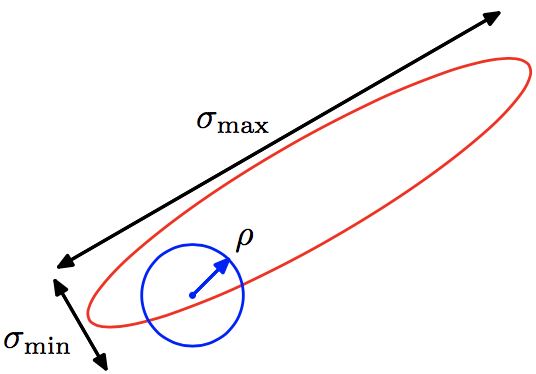
\includegraphics[scale=0.4]{gaussian_proposal.png}
  \caption{
    Gaussian proposal distribution.
  }
  \end{figure}
  \begin{itemize}
    \item If the variance is small, then the acceptance rate will be high,
    but the progress will be slow.
    \item However, if the variance is large, then the rejection rate will
    be high.
    \item The scale $\rho$ of the proposal distribution should be as large
    as possible without incurring high rejection rates.
    \item The number of steps needed to obtain independent samples will be
    of order
    \begin{equation}
      {( \sigma_{\textrm{max}} / \sigma_{\textrm{min}} )}^2
    \end{equation}
  \end{itemize}
\end{frame}


\subsection{MCMC: Gibbs Sampling}
\begin{frame}{Gibbs Sampling}
  \begin{figure}
  \centering
  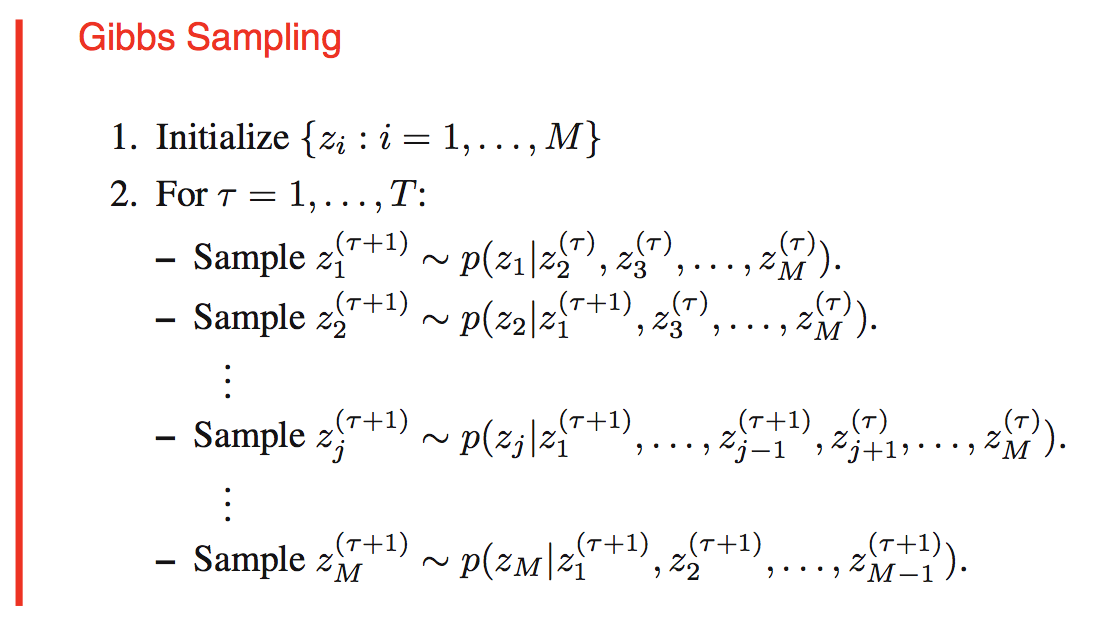
\includegraphics[scale=0.45]{gibbs_sampling.png}
  \caption{
    Gibbs Sampling.
  }
  \end{figure}
\end{frame}

\begin{frame}{Gibbs Sampling}
  \textbf{Acceptance function:}
  \begin{equation}
    A_(\mathbfit{z}^{*}, \mathbfit{z})
    =
      \frac{p(\mathbfit{z}^{*}) q_k(\mathbfit{z}|\mathbfit{z}^{*})}
      {p(\mathbfit{z}^{(\tau)}) q_k(\mathbfit{z}^{*}|\mathbfit{z})}
    =
    \frac{p(z_k^{*}|\mathbfit{z}_{-k}^{*}) p(\mathbfit{z}_{-k}^{*}) p(z_k|\mathbfit{z}_{-k}^{*})}
    {p(z_k|\mathbfit{z}_{-k}) p(\mathbfit{z}_{-k}) p(z_k^{*}|\mathbfit{z}_{-k})}
  \end{equation}
  where $\mathbfit{z}_{-k} = \mathbfit{z}^{*}_{-k}$
  \\[1.0\baselineskip]

  \textbf{Validation of equilibrium distribution $p$}
  \begin{equation}
    p(z_i = z_i^{(\tau + 1)}) = T(z_i = z_i^{(\tau)}, z_i = z_i^{(\tau + 1)}) p(z_i = z_i^{(\tau)})
  \end{equation}
  where $T = p(z_i|\mathbfit{z}_{-i})$. From this fact,
  \begin{equation}
    A_(\mathbfit{z}^{*}, \mathbfit{z}) = 1
  \end{equation}
  i.e., the Metropholis-Hastings steps are always accepted.
\end{frame}

\begin{frame}{Gibbs Sampling}
  \textbf{Random walk:}
  \begin{figure}
  \centering
  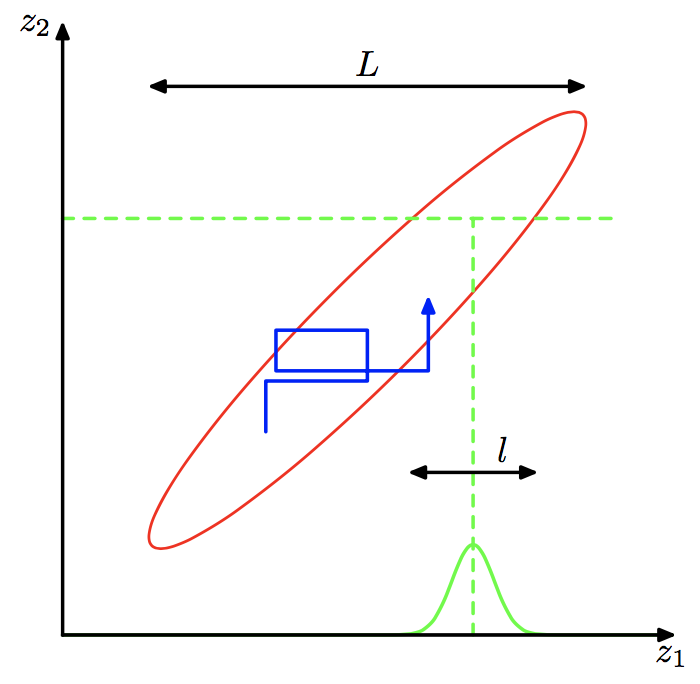
\includegraphics[scale=0.3]{gibbs_random_walk.png}
  \caption{
    Gibbs random walk
  }
  \end{figure}
  \begin{itemize}
    \item Because the state evolves according to a random walk,
    the number of steps needed to obtain independent samples
    from the distribution will be of order ${(L/l)}^2$.
    \item Reducing random walk: \textit{Over-relaxation}
  \end{itemize}
\end{frame}

\subsection{MCMC: Slice Sampling}
\begin{frame}{Slice Sampling}
  \textbf{Motivation}
  \begin{itemize}
    \item In Metropolis-Hastings Algorithm, If the step size is too small, the
    result is slow decorrelation due to random walk behaviour, whereas if it is
    too large the result is inefficiency due to a high rejection rate.
  \end{itemize}

  \textbf{Concept}
  \begin{itemize}
    \item adaptive step size that is automatically adjusted to match the
    characteristics of the distribution.
  \end{itemize}

  \begin{figure}
  \centering
  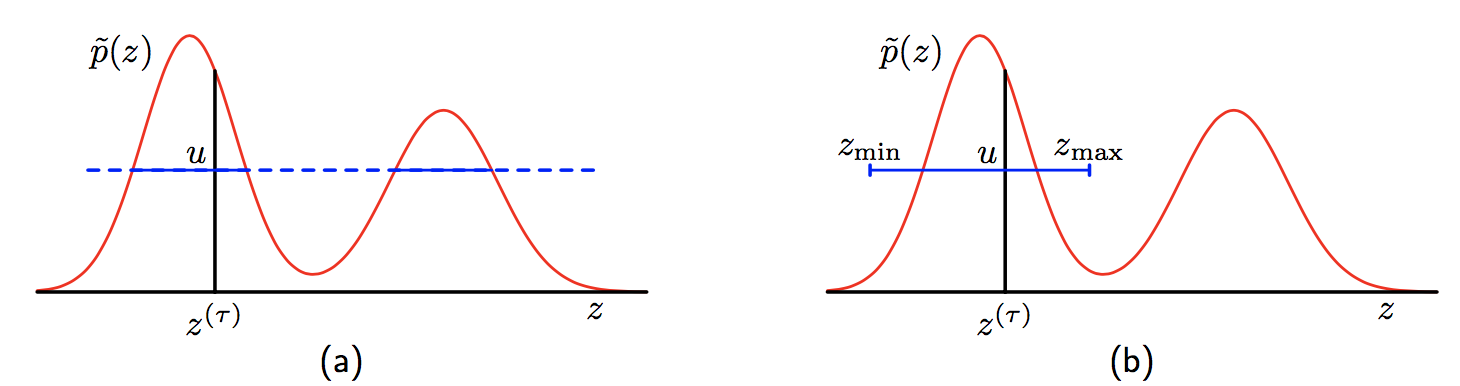
\includegraphics[scale=0.4]{slice_sampling.png}
  \caption{
    Slice Sampling.
  }
  \end{figure}
\end{frame}

\begin{frame}{Slice Sampling}
  \textbf{Augmented space $(z,u)$}
  \begin{itemize}
    \item Introduce additional variable $u$ so as to augment $z$ with $u$.
    \item Drawing samples from the joint $(z, u)$ space.
    \begin{equation}
      \hat{p}(z, u) =
      \left\{
      \begin{array}{ll}
        1/Z_p \quad & \textrm{if $0 \leq u \leq \tilde{p}(z)$} \\
        0     \quad & \textrm{otherwise.}
      \end{array}
      \right.
    \end{equation}
  \end{itemize}

  \textbf{Marginal distribution over $z$:}
  \begin{equation}
    \int \hat{p}(z, u) \mathrm{d}u
    = \int_{0}^{\tilde{p}(z)} \frac{1}{Z_p} \mathrm{d}u
    = \frac{\tilde{p}(z)}{Z_p} = p(z)
  \end{equation}
  \begin{itemize}
    \item We can sample from $p(z)$ by sampling from $\hat{p}(z, u)$ and
    then ignoring the $u$ values.
    \item This can be achieved by alternately sampling $z$ and $u$.
  \end{itemize}

  \textbf{Alternate sampling:}
  \begin{enumerate}
    \item Given $z$, evaluate $\tilde{p}(z)$.
    \item draw $u$ from $U(0, \tilde{p}(z))$.
    \item fix $u$, sample $z$ from $U(\{ z : \tilde{p}(z) > u \})$ \\
    (In practice, we can find the set $\{ z \}$ by iterative extension.)
  \end{enumerate}
\end{frame}

\section{Hybrid Monte Carlo Algorithm}
\begin{frame}{Dynamical systems}
  \textbf{Hamiltonian function:}
  \begin{equation}
    H(\mathbfit{z},\mathbfit{r}) = E(\mathbfit{z}) + K(\mathbfit{r})
  \end{equation}
  \begin{itemize}
    \item $H$ is constant:
    $\frac{\mathrm{d}H}{\mathrm{d}r} = 0$
    \\[1.0\baselineskip]
  \end{itemize}

  \textbf{Flow field:}
  \begin{equation}
    \mathbf{V} = \left(
      \frac{\mathrm{d}\mathbf{z}}{\mathrm{d}\tau},
      \frac{\mathrm{d}\mathbf{r}}{\mathrm{d}\tau}
    \right)
  \end{equation}
  \begin{itemize}
    \item The volume is invariant:
    $\textrm{div} \mathbf{V} = 0$
    \\[1.0\baselineskip]
  \end{itemize}

  \textbf{Joint distribution of $\mathbf{z}, \mathbf{r}$:}
  \begin{equation}
    p(\mathbf{z}, \mathbf{r}) =
    \frac{1}{Z_H} \exp{(-H(\mathbfit{z},\mathbfit{r}))}
  \end{equation}
  \begin{itemize}
    \item From the two results of conservation of volume and $H$,
    it follows that the Hamiltonian dynamics will leave
    $p(\mathbf{z}, \mathbf{r})$ \textbfit{invariant}.
  \end{itemize}
\end{frame}

\begin{frame}{Dynamical systems}
  \begin{itemize}
    \item Evolution under the Hamiltonian dynamics will not, however,
    sample ergodically from $p(\mathbf{z}, \mathbf{r})$ because
    the value of $H$ is constant.
    \item Noting that $\mathbf{z}$ and $\mathbf{r}$ are independent
    in the distribution and the conditional distribution
    $P(\mathbf{r} | \mathbf{z})$ is a Gaussian.
  \end{itemize}


\end{frame}

%%%%%%%%%%%%%%%%%%%%%%%%%%%%%%%%%%%%%%%%%%%%%%%%%%%%%%%%%%%%%%%%%%%%%
\end{document}
%%%%%%%%%%%%%%%%%%%%%%%%%%%%%%%%%%%%%%%%%%%%%%%% DOCUMENT start
